\usepackage{xcolor}
\usepackage{afterpage}
\usepackage{pifont,mdframed}
\usepackage{wrapfig}
\usepackage[bottom]{footmisc}

\makeatletter
\gdef\this@inputfilename{input.txt}
\gdef\this@outputfilename{output.txt}
\makeatother

\newcommand{\inputfile}{\texttt{input.txt}}
\newcommand{\outputfile}{\texttt{output.txt}}

\newenvironment{warning}
  {\par\begin{mdframed}[linewidth=2pt,linecolor=gray]%
    \begin{list}{}{\leftmargin=1cm
                   \labelwidth=\leftmargin}\item[\Large\ding{43}]}
  {\end{list}\end{mdframed}\par}

\begin{wrapfigure}{r}{5cm}
	\vspace{-1cm}
	\centering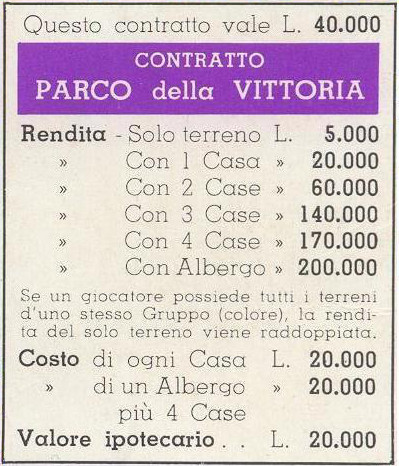
\includegraphics[width=.95\linewidth]{parco-vittoria.jpg}
	\vspace{-.5cm}
%	\caption{\small{Rappresentazione artistica della calcolatrice di Giorgio.}}
\end{wrapfigure}
L'ultima partita a Monopoly tra Gabriele e Giorgio è finita in tragedia dopo che Gabriele è stato costretto a ipotecare metà dei suoi terreni per coprire il costo dell'albergo di Giorgio in Parco della Vittoria.

Per evitare che la spiacevole situazione si ripeta un'altra volta, Gabriele sta mettendo in pratica gli insegnamenti del corso di ingegneria per costruire dei dadi robotici truccati. Il piano è molto astuto: i dadi sono progettati per fare in modo che Giorgio finisca sempre sulla casella più sfortunata, e che Gabriele si salvi sempre e paghi il minimo possibile ad ogni turno. Per raggiungere l'obiettivo, i dadi hanno all'interno un minuscolo giroscopio che permette loro di ruotare in modo da mostrare la faccia che decide Gabriele.

Gabriele non è uno sprovveduto, e sa che per non essere scoperto è necessario che nel lancio i dadi si muovano in modo realistico, compiendo molte rotazioni, all'apparenza casuali, ma che in realtà sono dettate dal software.

In questo momento Gabriele sta debuggando proprio questa parte di codice, verificando che i dadi compiano correttamente la sequenza di rotazioni imposta dal software. All'inizio della sequenza il dado si trova sempre nella posizione indicata in figura:

\begin{figure}[H]
	\centering\includegraphics[scale = 1.7]{asy_dadi/fig1.pdf}\\[2mm]
	Figura 1. Situazione iniziale del dado.
\end{figure}

Il driver che si occupa della rotazione accetta in input tre comandi: \texttt{X}, \texttt{Y}, e \texttt{Z}. Questi comandi hanno l'effetto di far compiere al dado una rotazione di 90 gradi rispetto all'asse scelto, in senso antiorario come mostrato dalle frecce grigie. Qui sotto sono rappresentati gli effetti dei comandi \texttt{X}, \texttt{Y}, e \texttt{Z} sul dado di Figura 1.

\begin{figure}[H]
	\centering
	\includegraphics[scale = .9]{asy_dadi/fig1_x.pdf}\hspace{1cm}
	\includegraphics[scale = .9]{asy_dadi/fig1_y.pdf}\hspace{1cm}
	\includegraphics[scale = .9]{asy_dadi/fig1_z.pdf}\\[2mm]
	Figura 2. Effetti dei comandi \texttt{X}, \texttt{Y}, e \texttt{Z} sul dado di Figura 1.
\end{figure}

Il driver supporta inoltre 3 comandi di interrogazione:
\begin{itemize}[nolistsep, itemsep=2mm]
	\item \texttt{T}: ritorna il valore sulla faccia superiore del dado, ovvero quella corrispondente al verso positivo dell'asse $z$;
	\item \texttt{F}: ritorna il valore sulla faccia frontale del dado, ovvero quella corrispondente al verso positivo dell'asse $y$;
	\item \texttt{R}: ritorna il valore sulla faccia destra del dado, ovvero quella corrispondente al verso positivo dell'asse $x$.
\end{itemize}

Aiuta Gabriele a debuggare i dadi truccati, scrivendo un software di simulazione che, ricevuta la sequenza di comandi inviati al dado, calcoli quali sono le risposte corrette alle varie richieste \texttt{T}, \texttt{F} e \texttt{R} inoltrate al driver.

\Implementation
Dovrai sottoporre esattamente un file con estensione \texttt{.c}, \texttt{.cpp} o \texttt{.pas}.

\begin{warning}
Tra gli allegati a questo task troverai un template (\texttt{dadi.c}, \texttt{dadi.cpp}, \texttt{dadi.pas}) con un esempio di implementazione da completare.
\end{warning}

Se sceglierai di utilizzare il template, dovrai implementare la seguente funzione:
\begin{center}\begin{tabularx}{\textwidth}{|c|X|}
\hline
C/C++  & \verb|void simula(int N, char C[], int R[]);|\\
\hline
Pascal & \verb|procedure simula(N: longint; var C: array of char; var R: array of longint);|\\
\hline
\end{tabularx}\end{center}
In cui:
\begin{itemize}[nolistsep]
  \item L'intero $N$ rappresenta il numero di comandi inoltrati al driver.
  \item L'array \texttt{C}, indicizzato da $0$ a $N-1$, contiene i comandi (un carattere tra \texttt{X, Y, Z, T, F, R}).
  \item La funzione dovrà riempire l'array di interi \texttt{R}, indicizzato da $0$ a $M-1$, dove $M$ rappresenza il numero di comandi di interrogazione (ovvero \texttt{T, F, R}). Nella posizione $i$ scrivere la risposta all'$i$-esimo comando di interrogazione.
\end{itemize}

\InputFile
Il file \inputfile{} è composto da due righe. La prima riga contiene l'unico intero $N$. La seconda riga contiene gli $N$ caratteri $C_i$, senza spazi.

\OutputFile
Il file \outputfile{} è composto da un'unica riga contenente gli $M$ interi di risposta.

% Assunzioni
\Constraints
\begin{itemize}[nolistsep, itemsep=2mm]
	\item $1 \le N \le 100\,000$.
	\item I comandi $C_i$ sono sempre un carattere tra \texttt{X, Y, Z, T, F} e \texttt{R}.
\end{itemize}

\Scoring
Il tuo programma verrà testato su diversi test case raggruppati in subtask.
Per ottenere il punteggio relativo ad un subtask, è necessario risolvere
correttamente tutti i test relativi ad esso.

\begin{itemize}[nolistsep,itemsep=2mm]
  \item \textbf{\makebox[2cm][l]{Subtask 1} [10 punti]}: Casi d'esempio.
  \item \textbf{\makebox[2cm][l]{Subtask 2} [20 punti]}: $N \leq 100$.
  \item \textbf{\makebox[2cm][l]{Subtask 3} [40 punti]}: $N \leq 1000$.
  \item \textbf{\makebox[2cm][l]{Subtask 4} [30 punti]}: Nessuna limitazione specifica.
\end{itemize}

% Esempi
\Examples
\begin{example}
\exmp{
9
XYYTZFXFR
}{%
2 3 2 1
}%
\end{example}
\begin{example}
\exmp{
10
TZZYXFRTXR
}{%
1 4 6 2 6
}%
\end{example}


\Explanation
Nel \textbf{primo caso di esempio} il dado subisce queste rotazioni:
\begin{figure}[H]
	\includegraphics[width = \textwidth]{asy_dadi/es1.pdf}
\end{figure}
Nel \textbf{secondo caso di esempio} il dado subisce queste rotazioni:
\begin{figure}[H]
	\includegraphics[width = \textwidth]{asy_dadi/es2.pdf}
\end{figure}